\documentclass[12pt,a4paper]{article}
\usepackage{amsmath, amssymb, geometry, booktabs, xcolor, hyperref,
            listings, pgfplots, tcolorbox, enumitem, fancyhdr, tikz, array}
\usepgfplotslibrary{fillbetween}
\geometry{margin=2.5cm}
\pgfplotsset{compat=1.18}
\tcbuselibrary{skins, breakable}

% Define custom environments
\newtcolorbox{curiositybox}[1]{colback=yellow!10, colframe=orange!80, title=#1, breakable}
\newtcolorbox{infobox}[1]{colback=blue!5, colframe=blue!60, title=#1, breakable}
\newtcolorbox{mistakebox}[1]{colback=red!5, colframe=red!60, title=#1, breakable}
\newtcolorbox{learnbox}[1]{colback=green!5, colframe=green!60, title=#1, breakable}

% Header and Footer
\pagestyle{fancy}
\fancyhf{}
\lhead{Series Expansions}
\rhead{Unit 3 -- LAC}
\cfoot{\thepage}

% Document Title Setup
\title{\textbf{Taylor's \& Maclaurin's Series, Approximation \& Error Estimation} \\ \large Unit 3 --- Single Variable Calculus and Series Expansions}
\author{Department of Mathematics}
\date{\today}

\begin{document}
\maketitle
\tableofcontents
\newpage

%=============================================================
\section{Real-World Engineering Hook}
%=============================================================

\begin{curiositybox}{Why Should an Engineer Care?}
Consider the firmware running on a microcontroller inside a drone's flight stabilisation unit.
The processor must compute \(\sin(\theta)\) hundreds of times per second to update motor speeds.
But floating-point trigonometry hardware does not exist on most embedded chips---instead, the
manufacturer stores a handful of polynomial coefficients in ROM derived from the first few terms
of the Maclaurin series for \(\sin x\).

If only \textbf{one term} is kept (\(\sin x \approx x\)), the approximation is fine for tiny
angles but catastrophically wrong beyond \(10^{\circ}\).
In a closed-loop feedback controller this mis-estimation feeds directly into the PID error signal:
the actuators receive wrong correction torques, oscillations grow, and the drone tumbles within
seconds.

On the other hand, keeping \textbf{fifteen terms} is mathematically perfect but wastes eight
precious microseconds per cycle---enough to miss the control deadline and produce the same crash
from latency rather than inaccuracy.

\medskip
\textbf{The engineering question is identical to the mathematical one:}
\emph{How many terms are enough, and how do we prove it?}
That is precisely what Taylor's theorem, Maclaurin's series, function approximation, and
error estimation answer.
\end{curiositybox}

%=============================================================
\section{Why This Topic Exists}
%=============================================================

\begin{center}
\begin{tabular}{>{\bfseries}p{5cm} p{9cm}}
\toprule
Theoretical Concept & Engineering Application / Consequence of Misunderstanding \\
\midrule
Taylor's Series with Remainder &
  Basis for numerical ODE solvers (Euler, RK4); ignoring the remainder causes
  accumulated truncation error that can make a simulation diverge over long time intervals. \\
\addlinespace
Maclaurin's Series &
  Standard expansions used in small-signal circuit analysis, Fourier approximation,
  optics (paraxial approximation), and signal processing filter design. \\
\addlinespace
Approximation of Functions &
  Linearisation of nonlinear dynamical systems in control engineering; misapplying a
  linear approximation far from the operating point destabilises the closed-loop response. \\
\addlinespace
Error Estimation &
  Determines acceptable precision in FEM computations, ADC quantisation tolerance,
  and sensor calibration---insufficient terms produce out-of-spec hardware. \\
\bottomrule
\end{tabular}
\end{center}

\begin{learnbox}{Core Learning Objective}
By the end of this lecture note, you will be able to:
\begin{itemize}[leftmargin=1.5em]
  \item Write the Taylor and Maclaurin series of any sufficiently differentiable function.
  \item Apply Lagrange's remainder to bound the truncation error rigorously.
  \item Use polynomial approximations to evaluate transcendental functions numerically.
  \item Determine the minimum number of terms required to meet a specified accuracy target.
\end{itemize}
\end{learnbox}

%=============================================================
\section{Intuition First \& Mathematical Definitions}
%=============================================================

\subsection{Taylor's Series with Remainder}

Imagine you are standing at the point \(x = a\) on the graph of a smooth function \(f\).
You can measure the height \(f(a)\), the slope \(f'(a)\), the curvature \(f''(a)\), and
all higher bending rates.
Taylor's theorem says: knowing all these local measurements lets you \emph{reconstruct the
entire curve}---the series is that reconstruction, and the remainder term tells you precisely
how much error you incur if you stop after finitely many terms.

\begin{infobox}{Taylor's Series with Remainder --- Formal Statement}
\textbf{Taylor's Series about \(x = a\):}
\[
  f(x) = f(a) + f'(a)(x-a) + \frac{f''(a)}{2!}(x-a)^2 + \cdots
         + \frac{f^{(n)}(a)}{n!}(x-a)^n + R_n(x)
\]
where the general term is \(\displaystyle\frac{f^{(k)}(a)}{k!}(x-a)^k\).

\medskip
\textbf{Lagrange Form of the Remainder:}
\[
  R_n(x) = \frac{f^{(n+1)}(c)}{(n+1)!}(x-a)^{n+1}
  \quad \text{for some } c \text{ strictly between } a \text{ and } x.
\]

\medskip
\textbf{Conditions for Validity:}
\begin{itemize}[leftmargin=1.5em]
  \item \(f\) must be \((n+1)\)-times differentiable on the open interval containing \(a\) and \(x\).
  \item The series converges to \(f(x)\) if and only if \(R_n(x) \to 0\) as \(n \to \infty\).
\end{itemize}

\medskip
\textbf{Key Insight:} The Lagrange remainder \(R_n(x)\) is not evaluated exactly (we do not know
\(c\)), but we can \emph{bound} it by replacing \(f^{(n+1)}(c)\) with its maximum on the interval.
\end{infobox}

\textbf{Worked Example 1.1 --- Expand \(e^x\) about \(x=1\) up to degree 4 and bound \(R_3\) on
\([1,\,1.5]\).}

\medskip
For \(f(x) = e^x\), every derivative satisfies \(f^{(k)}(x) = e^x\), so
\(f^{(k)}(1) = e\) for all \(k \geq 0\).

\[
  e^x = e + e(x-1) + \frac{e}{2!}(x-1)^2 + \frac{e}{3!}(x-1)^3
        + \frac{e}{4!}(x-1)^4 + R_4(x).
\]

For \(x \in [1,\,1.5]\), the fourth derivative is \(f^{(4)}(c)= e^c \leq e^{1.5}\).
We use \(e^{1.5} < 4.482\).

\textbf{Bounding \(R_3(x)\) (the error after the degree-3 polynomial):}
\[
  |R_3(x)| = \frac{|f^{(4)}(c)|}{4!}|x-1|^4
            \leq \frac{e^{1.5}}{24}(0.5)^4
            < \frac{4.482}{24} \times 0.0625
            = \frac{4.482 \times 0.0625}{24}
            = \frac{0.28013}{24}
            \approx 0.01167.
\]

So if we stop at the cubic term, the maximum error for any \(x \in [1,\,1.5]\) is less than
\(0.012\)---a useful engineering bound.

\subsection{Maclaurin's Series}

When the expansion point is \(a = 0\), the Taylor series simplifies beautifully: every
factor \((x-a)^k\) becomes just \(x^k\), and the coefficients only require derivatives
\emph{at the origin}.
This special case, called Maclaurin's series, produces the iconic polynomial forms of
\(e^x\), \(\sin x\), \(\cos x\), and so on, which engineers memorise and use everywhere.

\begin{infobox}{Maclaurin's Series --- Definition and Standard Expansions}
\textbf{Definition (Taylor's at \(a = 0\)):}
\[
  f(x) = f(0) + f'(0)\,x + \frac{f''(0)}{2!}\,x^2 + \frac{f'''(0)}{3!}\,x^3 + \cdots
         = \sum_{k=0}^{\infty} \frac{f^{(k)}(0)}{k!}\,x^k.
\]

\textbf{Standard Expansions:}
\begin{align*}
  e^x         &= 1 + x + \frac{x^2}{2!} + \frac{x^3}{3!} + \frac{x^4}{4!} + \cdots
                 \quad (\text{all } x,\; R = \infty) \\[4pt]
  \sin x      &= x - \frac{x^3}{3!} + \frac{x^5}{5!} - \frac{x^7}{7!} + \cdots
                 \quad (\text{all } x,\; R = \infty) \\[4pt]
  \cos x      &= 1 - \frac{x^2}{2!} + \frac{x^4}{4!} - \frac{x^6}{6!} + \cdots
                 \quad (\text{all } x,\; R = \infty) \\[4pt]
  \ln(1+x)    &= x - \frac{x^2}{2} + \frac{x^3}{3} - \frac{x^4}{4} + \cdots
                 \quad (-1 < x \leq 1,\; R = 1) \\[4pt]
  (1+x)^n     &= 1 + nx + \frac{n(n-1)}{2!}x^2 + \frac{n(n-1)(n-2)}{3!}x^3 + \cdots
                 \quad (|x| < 1 \text{ if } n \notin \mathbb{Z}_{\geq 0})
\end{align*}

\textbf{Radius of Convergence} \(R\): the series \(\sum a_k x^k\) converges absolutely for
\(|x| < R\) and diverges for \(|x| > R\), where
\(R = \lim_{k\to\infty} \left|\dfrac{a_k}{a_{k+1}}\right|\) (ratio test).
\end{infobox}

\textbf{Worked Example 2.1 --- Derive the Maclaurin series for \(e^x\) from first principles.}

Let \(f(x) = e^x\).
Compute successive derivatives and evaluate at \(x = 0\):
\[
  f(x) = e^x \;\Rightarrow\; f(0) = 1, \quad
  f'(x) = e^x \;\Rightarrow\; f'(0) = 1, \quad
  f''(x) = e^x \;\Rightarrow\; f''(0) = 1, \quad \ldots
\]
In general, \(f^{(k)}(0) = 1\) for every \(k \geq 0\).  Substituting into the Maclaurin
formula:
\[
  e^x = \sum_{k=0}^{\infty} \frac{1}{k!}\,x^k
      = 1 + x + \frac{x^2}{2} + \frac{x^3}{6} + \frac{x^4}{24} + \cdots
\]

\textbf{Verification at \(x = 1\):}
\[
  e^1 \approx 1 + 1 + 0.5 + 0.1\overline{6} + 0.04167 + 0.00833 + 0.00139
            = 2.71806 \quad (\text{exact: } e \approx 2.71828).
\]
Six terms already give four-decimal accuracy.

\medskip
\textbf{Worked Example 2.2 --- Expand \((1+x)^{1/2}\) up to the \(x^3\) term (Binomial Series).}

Set \(n = 1/2\) in the binomial expansion \((1+x)^n\):
\begin{align*}
  \text{Term 0:}\quad & 1 \\
  \text{Term 1:}\quad & \frac{1}{2}\,x \\
  \text{Term 2:}\quad & \frac{\frac{1}{2}\!\left(\frac{1}{2}-1\right)}{2!}\,x^2
                       = \frac{\frac{1}{2}\cdot\left(-\frac{1}{2}\right)}{2}\,x^2
                       = -\frac{1}{8}\,x^2 \\
  \text{Term 3:}\quad & \frac{\frac{1}{2}\!\left(-\frac{1}{2}\right)\!\left(-\frac{3}{2}\right)}{3!}\,x^3
                       = \frac{\frac{3}{8}}{6}\,x^3
                       = \frac{1}{16}\,x^3
\end{align*}
Therefore:
\[
  \sqrt{1+x} = 1 + \frac{x}{2} - \frac{x^2}{8} + \frac{x^3}{16} - \cdots
  \qquad (|x| < 1).
\]

\subsection{Approximation of Functions}

The Taylor and Maclaurin series give infinitely many terms, but in practice we stop after
just one or two.
Stopping after the linear term gives the \emph{tangent-line approximation}---the simplest
tool engineers use to ``linearise'' a curved relationship near an operating point.
The quadratic term adds curvature correction when the linear approximation is not good enough.

\begin{infobox}{Polynomial Approximations --- Formulas and Validity}
\textbf{Linear (First-Degree) Approximation about \(x = a\):}
\[
  f(x) \approx f(a) + f'(a)(x - a).
\]
This is the equation of the tangent line to \(f\) at \(x = a\).

\medskip
\textbf{Quadratic (Second-Degree) Approximation:}
\[
  f(x) \approx f(a) + f'(a)(x-a) + \frac{f''(a)}{2}(x-a)^2.
\]

\medskip
\textbf{\(n\)-th Degree Polynomial Approximation:}
\[
  P_n(x) = \sum_{k=0}^{n} \frac{f^{(k)}(a)}{k!}(x-a)^k.
\]

\textbf{Conditions for a Good Approximation:}
\begin{itemize}[leftmargin=1.5em]
  \item \(x\) must be \emph{close} to \(a\) so that \(|x - a|\) is small.
  \item The remainder \(|R_n(x)|\) must be smaller than the required tolerance \(\varepsilon\).
  \item Higher-degree terms become negligible only when \(|x-a|^k / k!\) decreases rapidly,
        which requires \(|x - a| < 1\) at least as a rule of thumb.
\end{itemize}

\textbf{Geometric View:} The linear approximation is the tangent line; the quadratic approximation
is an osculating parabola---it matches \(f\) in value, slope, and curvature at \(x = a\).
\end{infobox}

\textbf{Worked Example 3.1 --- Estimate \(\sin(31^{\circ})\) using linear approximation; compare
with exact.}

Convert: \(31^{\circ} = \dfrac{31\pi}{180}\) rad.
Choose expansion point \(a = 30^{\circ} = \dfrac{\pi}{6}\) rad (known exact values).

\[
  f(x) = \sin x, \quad f(a) = \sin\!\tfrac{\pi}{6} = 0.5, \quad
  f'(a) = \cos\!\tfrac{\pi}{6} = \tfrac{\sqrt{3}}{2} \approx 0.86603.
\]

\[
  x - a = \frac{31\pi}{180} - \frac{\pi}{6}
        = \frac{31\pi - 30\pi}{180}
        = \frac{\pi}{180} \approx 0.017453 \text{ rad}.
\]

\textbf{Linear approximation:}
\[
  \sin(31^{\circ}) \approx 0.5 + 0.86603 \times 0.017453
                         = 0.5 + 0.015116
                         = 0.51512.
\]

\textbf{Exact value:} \(\sin(31^{\circ}) = 0.51504\) (to 5 d.p.).

\textbf{Absolute error:} \(|0.51512 - 0.51504| = 0.00008\) --- less than \(0.02\%\).

\medskip
\textbf{Worked Example 3.2 --- Approximate \(\sqrt{1.05}\) for manufacturing tolerance
calculations.}

Let \(f(x) = \sqrt{x} = x^{1/2}\), expand about \(a = 1\):
\[
  f(1) = 1, \quad f'(x) = \tfrac{1}{2}x^{-1/2} \;\Rightarrow\; f'(1) = 0.5.
\]

\textbf{Linear approximation at \(x = 1.05\):}
\[
  \sqrt{1.05} \approx 1 + 0.5(1.05 - 1) = 1 + 0.5 \times 0.05 = 1 + 0.025 = 1.025.
\]

\textbf{Exact value:} \(\sqrt{1.05} = 1.02470\) (5 d.p.).

\textbf{Error:} \(|1.025 - 1.02470| = 0.00030\), which is \(0.029\%\)---well within typical
manufacturing tolerances of \(0.1\%\).

\subsection{Error Estimation}

When we truncate an infinite series at term \(n\), we introduce a \emph{truncation error}.
Lagrange's remainder gives us a watertight upper bound on this error without needing to know the
mysterious intermediate point \(c\)---we simply bound the \((n+1)\)-th derivative over the
entire interval of interest.

\begin{infobox}{Error Estimation --- Lagrange Remainder and Algorithm}
\textbf{Lagrange Remainder (restated for error bounding):}
\[
  |R_n(x)| = \left|\frac{f^{(n+1)}(c)}{(n+1)!}(x-a)^{n+1}\right|
            \leq \frac{M_{n+1}}{(n+1)!}|x-a|^{n+1},
\]
where \(M_{n+1} = \max_{t \in [\min(a,x),\, \max(a,x)]}|f^{(n+1)}(t)|\).

\medskip
\textbf{Algorithm: Choose \(n\) for Target Accuracy \(\varepsilon\):}
\begin{enumerate}[leftmargin=2em, label=\textbf{Step \arabic*.}]
  \item Set \(n = 1\).
  \item Compute \(M_{n+1} = \max |f^{(n+1)}|\) on the relevant interval.
  \item Evaluate the bound \(B_n = \dfrac{M_{n+1}}{(n+1)!}|x-a|^{n+1}\).
  \item If \(B_n \leq \varepsilon\): stop; use \(n\) terms.
  \item Otherwise: set \(n \leftarrow n+1\) and return to Step 2.
\end{enumerate}

\medskip
\textbf{Key Fact:} Because \(1/k!\) decreases faster than any exponential, the algorithm
always terminates for analytic functions over bounded intervals.
\end{infobox}

\textbf{Worked Example 4.1 --- How many terms of the Maclaurin series for \(e^x\) give accuracy
\(0.0001\) on \([0,1]\)?}

Here \(a = 0\), \(x \in [0,1]\), \(f(x) = e^x\).
Every derivative is \(e^x\), so \(M_{n+1} = e^1 < 2.71828\) on \([0,1]\).
The bound on the error after \(n\) terms (i.e., the polynomial \(P_{n-1}\) of degree \(n-1\)) is:
\[
  |R_{n-1}(x)| \leq \frac{e}{n!} \cdot 1^n = \frac{e}{n!}.
\]

\begin{center}
\begin{tabular}{ccc}
\toprule
\(n\) & \(n!\) & \(e / n!\) \\
\midrule
1 & 1 & 2.71828 \\
2 & 2 & 1.35914 \\
3 & 6 & 0.45305 \\
4 & 24 & 0.11326 \\
5 & 120 & 0.02265 \\
6 & 720 & 0.003775 \\
7 & 5040 & 0.000540 \\
8 & 40320 & 0.0000674 $< 0.0001$ \\
\bottomrule
\end{tabular}
\end{center}

At \(n = 8\): \(e/8! = e/40320 \approx 6.74 \times 10^{-5} < 0.0001\).

\textbf{Conclusion:} We need the first \textbf{8 terms} (degree-7 polynomial) to guarantee
accuracy \(0.0001\) for all \(x \in [0,1]\).

%=============================================================
\section{Visual Artifacts \& Geometric Interpretation}
%=============================================================

\subsection*{Figure 1: Maclaurin Polynomials for \(\sin x\) --- Convergence on \([-\pi, \pi]\)}

\begin{center}
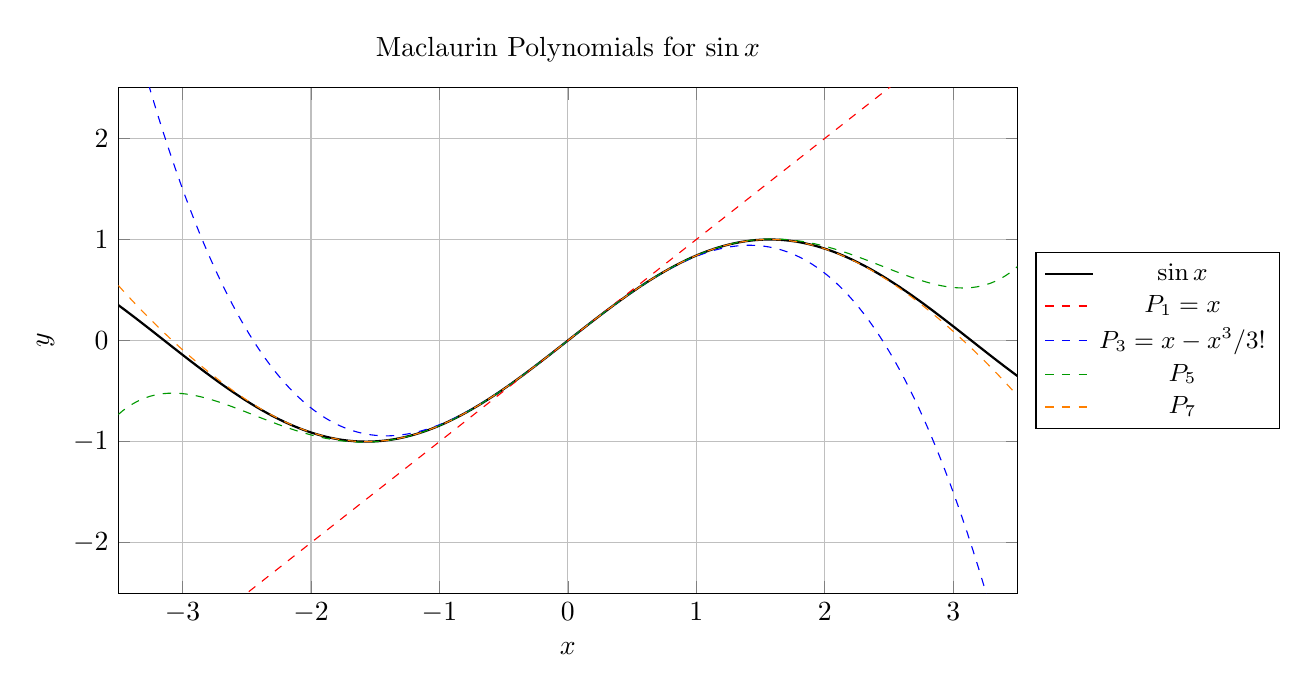
\begin{tikzpicture}
\begin{axis}[
  width=13cm, height=8cm,
  xmin=-3.5, xmax=3.5,
  ymin=-2.5, ymax=2.5,
  xlabel={$x$},
  ylabel={$y$},
  title={Maclaurin Polynomials for $\sin x$},
  legend style={at={(1.02,0.5)}, anchor=west, font=\small},
  grid=major,
  samples=200
]
\addplot[thick, black, domain=-3.5:3.5] {sin(deg(x))};
\addlegendentry{$\sin x$}
\addplot[red, dashed, domain=-3.5:3.5] {x};
\addlegendentry{$P_1 = x$}
\addplot[blue, dashed, domain=-3.5:3.5] {x - x^3/6};
\addlegendentry{$P_3 = x - x^3/3!$}
\addplot[green!60!black, dashed, domain=-3.5:3.5] {x - x^3/6 + x^5/120};
\addlegendentry{$P_5$}
\addplot[orange, dashed, domain=-3.5:3.5] {x - x^3/6 + x^5/120 - x^7/5040};
\addlegendentry{$P_7$}
\end{axis}
\end{tikzpicture}
\end{center}

The higher the degree, the longer the polynomial ``hugs'' the sine curve before diverging.
By degree 7, the approximation is visually indistinguishable from \(\sin x\) on \([-\pi,\pi]\).

\subsection*{Figure 2: Maclaurin Approximations for \(e^x\) on \([0,1]\) with Error Shading}

\begin{center}
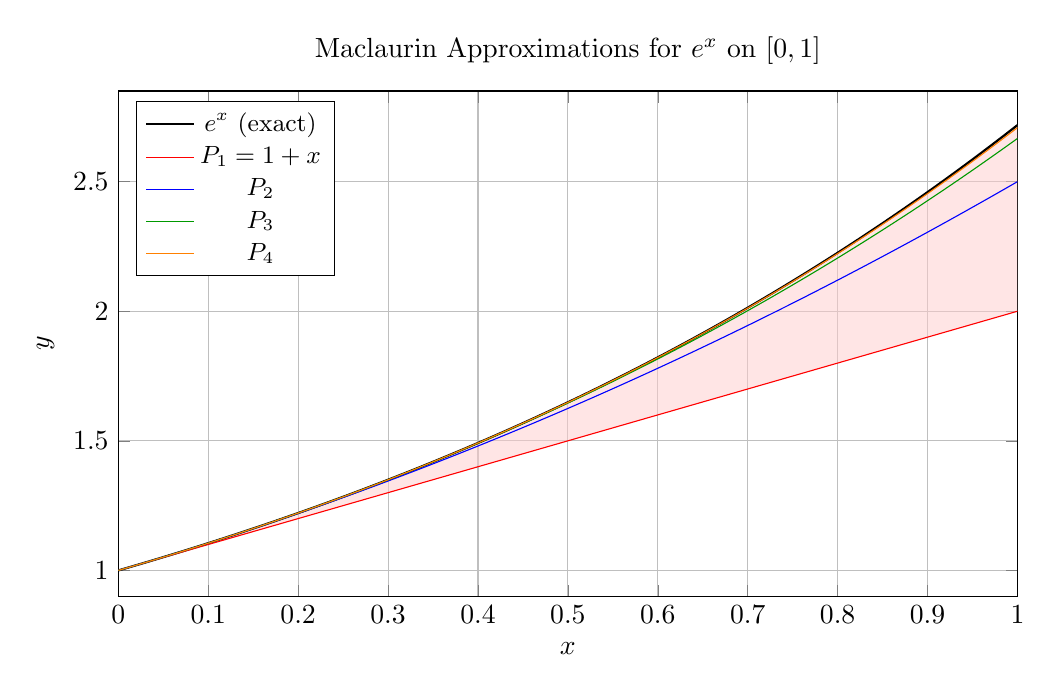
\begin{tikzpicture}
\begin{axis}[
  width=13cm, height=8cm,
  xmin=0, xmax=1,
  ymin=0.9, ymax=2.85,
  xlabel={$x$},
  ylabel={$y$},
  title={Maclaurin Approximations for $e^x$ on $[0,1]$},
  legend style={at={(0.02,0.98)}, anchor=north west, font=\small},
  grid=major,
  samples=200
]
\addplot[name path=exact, thick, black, domain=0:1] {exp(x)};
\addlegendentry{$e^x$ (exact)}
\addplot[name path=p1, red, domain=0:1] {1+x};
\addlegendentry{$P_1 = 1+x$}
\addplot[name path=p2, blue, domain=0:1] {1+x+x^2/2};
\addlegendentry{$P_2$}
\addplot[name path=p3, green!60!black, domain=0:1] {1+x+x^2/2+x^3/6};
\addlegendentry{$P_3$}
\addplot[name path=p4, orange, domain=0:1] {1+x+x^2/2+x^3/6+x^4/24};
\addlegendentry{$P_4$}
\addplot[red!20, opacity=0.5] fill between[of=exact and p1];
\end{axis}
\end{tikzpicture}
\end{center}

The shaded region between the exact curve and \(P_1\) illustrates the magnitude of the
truncation error.
Adding more terms visibly closes this gap.

\subsection*{Figure 3: Error Estimation Flowchart}

\begin{center}
\begin{tikzpicture}[
  node distance=1.4cm,
  box/.style={rectangle, draw, rounded corners, fill=blue!10,
              text width=6cm, align=center, minimum height=0.8cm},
  decision/.style={diamond, draw, fill=orange!20,
                   text width=3.5cm, align=center, aspect=2},
  arrow/.style={->, thick}
]
\node[box] (start) {Start: choose target accuracy $\varepsilon$, set $n = 1$};
\node[box, below=of start] (M) {Compute $M_{n+1} = \max|f^{(n+1)}|$ on interval};
\node[box, below=of M] (B) {Compute bound $B_n = \dfrac{M_{n+1}}{(n+1)!}|x-a|^{n+1}$};
\node[decision, below=of B] (check) {$B_n \leq \varepsilon$?};
\node[box, below=of check] (done) {Use $n$ terms of the Taylor/Maclaurin series};
\node[box, right=3cm of check] (inc) {Increment $n \leftarrow n+1$};

\draw[arrow] (start) -- (M);
\draw[arrow] (M) -- (B);
\draw[arrow] (B) -- (check);
\draw[arrow] (check) -- node[left]{\textbf{Yes}} (done);
\draw[arrow] (check) -- node[above]{\textbf{No}} (inc);
\draw[arrow] (inc) |- (M);
\end{tikzpicture}
\end{center}

%=============================================================
\section{Step-by-Step Algorithmic Workflow}
%=============================================================

\begin{tcolorbox}[colback=gray!5, colframe=gray!50, title=\textbf{Master Workflow for Series Expansions}, breakable]

\textbf{Workflow A: Writing a Taylor Series}
\begin{enumerate}[leftmargin=2em]
  \item Identify the expansion centre \(a\) and the required degree \(n\).
  \item Compute \(f(a),\; f'(a),\; f''(a),\; \ldots,\; f^{(n)}(a)\) --- evaluate each derivative at \(x = a\).
  \item Write the partial sum: \(P_n(x) = \sum_{k=0}^{n}\dfrac{f^{(k)}(a)}{k!}(x-a)^k\).
  \item Attach the Lagrange remainder: \(R_n(x) = \dfrac{f^{(n+1)}(c)}{(n+1)!}(x-a)^{n+1}\).
  \item State the interval of convergence.
\end{enumerate}

\medskip
\textbf{Workflow B: Maclaurin Series}
\begin{enumerate}[leftmargin=2em]
  \item Set \(a = 0\) in Workflow A.
  \item If \(f\) is one of the standard functions (\(e^x\), \(\sin x\), \(\cos x\), \(\ln(1+x)\), \((1+x)^n\)),
        read the series directly from the standard table.
  \item Verify radius of convergence before using the result.
\end{enumerate}

\medskip
\textbf{Workflow C: Function Approximation}
\begin{enumerate}[leftmargin=2em]
  \item Choose degree \(n\) (often \(n=1\) for engineering linearisation).
  \item Choose expansion point \(a\) close to the evaluation point \(x\).
  \item Evaluate \(P_n(x)\).
  \item Compute the error bound \(|R_n(x)|\) to confirm adequacy.
\end{enumerate}

\medskip
\textbf{Workflow D: Error Bounding}
\begin{enumerate}[leftmargin=2em]
  \item Identify the degree \(n\) of the approximation being used.
  \item Find \(M_{n+1} = \max |f^{(n+1)}|\) on the closed interval \([\min(a,x),\max(a,x)]\).
  \item Compute \(|R_n| \leq \dfrac{M_{n+1}}{(n+1)!}|x-a|^{n+1}\).
  \item Compare with required \(\varepsilon\); if \(|R_n| > \varepsilon\), increase \(n\) and repeat.
\end{enumerate}
\end{tcolorbox}

%=============================================================
\section{Fully Worked Step-by-Step Numerical Examples}
%=============================================================

\subsection*{Example 1 --- Taylor Expansion of \(\ln x\) about \(x=1\) up to Degree 4}

\textbf{Given:} \(f(x) = \ln x\), expand about \(a = 1\), degree \(n = 4\).
Bound the Lagrange remainder for \(x = 1.2\).

\medskip
\textbf{Step 1: Compute derivatives and evaluate at \(a = 1\).}
\begin{align*}
  f(x)    &= \ln x,                \quad f(1)    = 0. \\
  f'(x)   &= x^{-1},               \quad f'(1)   = 1. \\
  f''(x)  &= -x^{-2},              \quad f''(1)  = -1. \\
  f'''(x) &= 2x^{-3},              \quad f'''(1) = 2. \\
  f^{(4)}(x) &= -6x^{-4},         \quad f^{(4)}(1) = -6.
\end{align*}

\textbf{Step 2: Write the degree-4 Taylor polynomial.}
\[
  P_4(x) = 0 + 1\cdot(x-1) + \frac{-1}{2!}(x-1)^2 + \frac{2}{3!}(x-1)^3
           + \frac{-6}{4!}(x-1)^4.
\]
\[
  P_4(x) = (x-1) - \frac{(x-1)^2}{2} + \frac{(x-1)^3}{3} - \frac{(x-1)^4}{4}.
\]

\textbf{Step 3: Verify at \(x = 1.2\).}
Let \(h = x - 1 = 0.2\):
\[
  P_4(1.2) = 0.2 - \frac{0.04}{2} + \frac{0.008}{3} - \frac{0.0016}{4}
           = 0.2 - 0.02 + 0.002\overline{6} - 0.0004
           = 0.18227.
\]
Exact: \(\ln(1.2) = 0.18232\) (5 d.p.).  Error \(= 0.00005\).

\textbf{Step 4: Bound \(|R_4(x)|\) at \(x = 1.2\).}
\[
  f^{(5)}(x) = 24x^{-5}, \quad
  M_5 = \max_{t \in [1,1.2]} 24t^{-5} = 24 \cdot 1^{-5} = 24.
\]
\[
  |R_4(1.2)| \leq \frac{24}{5!}(0.2)^5
             = \frac{24}{120} \times 0.00032
             = 0.2 \times 0.00032
             = 0.000064.
\]
The computed error \(0.00005\) is indeed within this bound.

\begin{learnbox}{Insight from Example 1}
The Taylor expansion of \(\ln x\) about \(x=1\) is in powers of \((x-1)\), not
\(x\).
Always verify that the expansion variable \((x-a)\) is small before trusting a
low-degree approximation.
\end{learnbox}

\subsection*{Example 2 --- Maclaurin Series for \(e^{-x^2}\)}

\textbf{Why this function?} \(e^{-x^2}\) has no elementary antiderivative---the error function
\(\mathrm{erf}(x)\) used in probability and signal processing \emph{is} defined as its integral.
The Maclaurin series is the only closed-form computational tool.

\textbf{Step 1:} Use the known series for \(e^u = \sum_{k=0}^{\infty}\dfrac{u^k}{k!}\).

\textbf{Step 2:} Substitute \(u = -x^2\):
\[
  e^{-x^2} = \sum_{k=0}^{\infty} \frac{(-x^2)^k}{k!}
           = \sum_{k=0}^{\infty} \frac{(-1)^k x^{2k}}{k!}.
\]

\textbf{Step 3:} Write out the first five terms:
\[
  e^{-x^2} = 1 - x^2 + \frac{x^4}{2} - \frac{x^6}{6} + \frac{x^8}{24} - \cdots
\]

\textbf{Step 4:} Integrate to get the error function approximation:
\[
  \int_0^x e^{-t^2}\,dt \approx x - \frac{x^3}{3} + \frac{x^5}{10} - \frac{x^7}{42}
                               + \frac{x^9}{216} - \cdots
\]

\begin{learnbox}{Insight from Example 2}
Substitution into a known Maclaurin series (here \(e^u\) with \(u=-x^2\)) is
far faster than differentiating from scratch.
The resulting series converges for all \(x\) because \(e^u\) converges
everywhere.
\end{learnbox}

\subsection*{Example 3 --- Engineering: Small-Angle Approximation for Beam Deflection}

\textbf{Problem:} A structural engineer must evaluate \(\sin(0.05\,\text{rad})\) appearing in a
small-angle beam deflection formula.
Use the Maclaurin series and confirm that 2 terms give less than \(0.0001\%\) error.

\textbf{Step 1: Two-term Maclaurin approximation.}
\[
  \sin x \approx x - \frac{x^3}{6}, \quad x = 0.05.
\]
\[
  \sin(0.05) \approx 0.05 - \frac{(0.05)^3}{6}
             = 0.05 - \frac{0.000125}{6}
             = 0.05 - 0.00002083
             = 0.04997917.
\]

\textbf{Step 2: Exact value.}
\(\sin(0.05) = 0.0499792\) (7 d.p.).

\textbf{Step 3: Error bound (remainder after 2 terms, \(n=2\)).}
The next term is the \(x^5/5!\) term.
\(|f^{(5)}(c)| = |\cos c| \leq 1\) for all \(c\).
\[
  |R_2| \leq \frac{1}{5!}(0.05)^5
          = \frac{1}{120}\times 3.125\times10^{-7}
          = 2.60\times10^{-9}.
\]

\textbf{Step 4: Percentage error.}
\[
  \frac{2.60\times10^{-9}}{0.05} \times 100\%
  = 5.21\times10^{-6}\% \ll 0.0001\%.
\]

\textbf{Engineering interpretation:} Two terms are more than sufficient for beam
deflection calculations where measurement uncertainties of the loading already exceed
\(0.1\%\).

\begin{learnbox}{Insight from Example 3}
For \(x < 0.1\) rad, \(\sin x \approx x\) alone gives errors under \(0.17\%\).
Adding the cubic correction term reduces this to below \(3\times10^{-4}\%\).
Most engineering ``small angle'' analyses require \(x < 0.3\) rad for the single-term
approximation to be acceptable.
\end{learnbox}

\subsection*{Example 4 --- Minimum Terms of Maclaurin Series for \(\cos(0.5)\) with Error
\(< 10^{-6}\)}

\textbf{Step 1: Identify the series.}
\[
  \cos x = \sum_{k=0}^{\infty}\frac{(-1)^k x^{2k}}{(2k)!}
         = 1 - \frac{x^2}{2!} + \frac{x^4}{4!} - \frac{x^6}{6!} + \cdots
\]

\textbf{Step 2: Remainder after \(n\) terms (i.e., using terms up to \(x^{2(n-1)}\)).}
For the alternating series for \(\cos x\), the error is bounded by the first omitted term:
\[
  |R| \leq \frac{|x|^{2n}}{(2n)!}.
\]
with \(x = 0.5\).

\textbf{Step 3: Tabulate.}
\begin{center}
\begin{tabular}{ccc}
\toprule
Terms used & Last exponent & Error bound \\
\midrule
1 (only $1$)               & $x^0$ & $(0.5)^2/2! = 0.125$              \\
2 (up to $x^2$)            & $x^2$ & $(0.5)^4/4! = 0.002604$           \\
3 (up to $x^4$)            & $x^4$ & $(0.5)^6/6! = 2.17\times10^{-5}$  \\
4 (up to $x^6$)            & $x^6$ & $(0.5)^8/8! = 9.69\times10^{-8} < 10^{-6}$ \\
\bottomrule
\end{tabular}
\end{center}

\textbf{Step 4: Compute.}
At 4 terms (up to \(x^6\)):
\[
  \cos(0.5) \approx 1 - \frac{0.25}{2} + \frac{0.0625}{24} - \frac{0.015625}{720}
           = 1 - 0.125 + 0.0026042 - 0.0000217
           = 0.8775825.
\]
Exact: \(\cos(0.5) = 0.8775826\).  Error \(= 1\times10^{-7} < 10^{-6}\). \checkmark

\textbf{Conclusion: 4 terms suffice.}

\begin{learnbox}{Insight from Example 4}
For alternating series with decreasing terms, the error is always less than the
first omitted term.
This is much sharper than the general Lagrange bound and saves computation in
practice.
\end{learnbox}

%=============================================================
\section{Tabular Comparison / Workflow Reference}
%=============================================================

\subsection*{Standard Maclaurin Series Quick Reference}

\begin{center}
\begin{tabular}{p{3cm} p{7.5cm} p{3cm}}
\toprule
\textbf{Function} & \textbf{Maclaurin Series} & \textbf{Radius of Convergence} \\
\midrule
$e^x$ &
$1 + x + \dfrac{x^2}{2!} + \dfrac{x^3}{3!} + \dfrac{x^4}{4!} + \cdots$ &
$R = \infty$ \\[8pt]
$\sin x$ &
$x - \dfrac{x^3}{3!} + \dfrac{x^5}{5!} - \dfrac{x^7}{7!} + \cdots$ &
$R = \infty$ \\[8pt]
$\cos x$ &
$1 - \dfrac{x^2}{2!} + \dfrac{x^4}{4!} - \dfrac{x^6}{6!} + \cdots$ &
$R = \infty$ \\[8pt]
$\ln(1+x)$ &
$x - \dfrac{x^2}{2} + \dfrac{x^3}{3} - \dfrac{x^4}{4} + \cdots$ &
$-1 < x \leq 1$ \\[8pt]
$(1+x)^n$ &
$1 + nx + \dfrac{n(n-1)}{2!}x^2 + \dfrac{n(n-1)(n-2)}{3!}x^3 + \cdots$ &
$|x| < 1$ (non-integer $n$) \\[8pt]
$\tan^{-1} x$ &
$x - \dfrac{x^3}{3} + \dfrac{x^5}{5} - \dfrac{x^7}{7} + \cdots$ &
$|x| \leq 1$ \\[8pt]
$\sinh x$ &
$x + \dfrac{x^3}{3!} + \dfrac{x^5}{5!} + \dfrac{x^7}{7!} + \cdots$ &
$R = \infty$ \\[8pt]
$\cosh x$ &
$1 + \dfrac{x^2}{2!} + \dfrac{x^4}{4!} + \dfrac{x^6}{6!} + \cdots$ &
$R = \infty$ \\
\bottomrule
\end{tabular}
\end{center}

\subsection*{Remainder Forms at a Glance}

\begin{center}
\begin{tabular}{lll}
\toprule
\textbf{Remainder Form} & \textbf{Formula} & \textbf{Best Used When} \\
\midrule
Lagrange & $\dfrac{f^{(n+1)}(c)}{(n+1)!}(x-a)^{n+1}$ & General upper bound \\[6pt]
Alternating Series & $\leq |$first omitted term$|$ & Alternating series only \\[6pt]
Big-O notation & $O((x-a)^{n+1})$ & Asymptotic analysis, limit problems \\
\bottomrule
\end{tabular}
\end{center}

%=============================================================
\section{Common Student Mistakes \& Pitfalls}
%=============================================================

\begin{mistakebox}{Common Mistakes in Series Expansions}
\begin{tabular}{>{\raggedright}p{4.5cm} >{\raggedright}p{4cm} p{5.5cm}}
\toprule
\textbf{Mistake Made} & \textbf{Why Students Do It} & \textbf{Correct Approach} \\
\midrule
Confusing expansion centre \(a\) with evaluation point \(x\) &
Variable notation confusion between \(a\) and \(x\) &
\(a\) is the point where derivatives are evaluated; \(x\) is where the polynomial is
computed; \(R_n\) depends on \((x-a)\). \\[6pt]
Using the \(n\)-th derivative instead of the \((n+1)\)-th in the remainder formula &
The polynomial ends at \(f^{(n)}\), so students incorrectly use the same derivative for
the error &
Lagrange remainder \(R_n\) uses \(f^{(n+1)}\) --- always one derivative beyond the last
term included. \\[6pt]
Applying Maclaurin series outside its radius of convergence &
Forgetting to check convergence before substituting \(x\) &
Always state and verify the radius of convergence \(R\); never evaluate outside $|x| < R$
(e.g., \(\ln(1+x)\) diverges for \(|x| > 1\)). \\[6pt]
Trusting a linear approximation far from \(a\) &
Intuitive over-confidence in the tangent-line picture &
Compute the error bound first; if \(|R_1| >\) tolerance, include the quadratic or higher
term. \\[6pt]
Forgetting the factorial denominator \(k!\) in coefficients &
Writing \(f^{(k)}(a)(x-a)^k\) instead of \(\dfrac{f^{(k)}(a)}{k!}(x-a)^k\) &
Every coefficient in the Taylor series carries \(1/k!\); a missing factorial can
off by a factor of 6 or more for degree-3 terms. \\[6pt]
Treating the series for \(e^{-x^2}\) as needing new derivative calculations &
Not recognising that substitution into a known series is valid &
Substitute \(u = -x^2\) directly into the series for \(e^u\); no differentiation
needed. \\
\bottomrule
\end{tabular}
\end{mistakebox}

%=============================================================
\section{Comprehensive Assessment Suite}
%=============================================================

\subsection*{Viva-Voce Questions}

\begin{enumerate}[leftmargin=2em, label=\textbf{V\arabic*.}]

\item \textbf{[Taylor's Series]} State Taylor's Theorem with Lagrange Remainder in full mathematical
  form, including all conditions on the function \(f\).

\item \textbf{[Taylor's Series]} What is the physical/geometric significance of the remainder term
  \(R_n(x)\)? Why can we not compute it exactly in general?

\item \textbf{[Taylor's Series]} If \(f(x) = \cos x\), write the Taylor series about
  \(a = \pi/2\). What is the first non-zero coefficient?

\item \textbf{[Maclaurin's Series]} Is Maclaurin's series a special case of Taylor's series?
  Justify your answer with a mathematical argument.

\item \textbf{[Maclaurin's Series]} Write the Maclaurin series for \(\sin x\) and \(\cos x\)
  from first principles, computing at least the first four non-zero terms of each.

\item \textbf{[Maclaurin's Series]} Why does the Maclaurin series for \(\ln(1+x)\) converge only
  for \(-1 < x \leq 1\)? What happens at \(x = -1\)?

\item \textbf{[Approximation]} When is a linear approximation \(f(x) \approx f(a) + f'(a)(x-a)\)
  a valid engineering tool? Give two conditions that must hold.

\item \textbf{[Approximation]} In control engineering, why is linearisation (linear approximation)
  of a nonlinear plant used? What goes wrong if the system moves far from the operating point?

\item \textbf{[Error Estimation]} State the Lagrange form of the remainder and explain each symbol
  in the formula.

\item \textbf{[Error Estimation]} How do you determine the minimum value of \(n\) such that the
  Maclaurin series for \(e^x\) approximates \(e^x\) with error less than \(10^{-4}\) on
  \([0,2]\)? Outline the method step by step.

\end{enumerate}

\subsection*{Descriptive Problems}

\begin{enumerate}[leftmargin=2em, label=\textbf{D\arabic*.}]

\item Expand \(f(x) = \cos x\) as a Taylor series about \(a = \pi/3\) up to the term containing
  \((x - \pi/3)^4\). Evaluate the polynomial at \(x = \pi/3 + 0.1\) and bound the error using the
  Lagrange remainder.
  \textit{Hint: Derivatives of \(\cos x\) cycle through \(\cos x, -\sin x, -\cos x, \sin x\).}

\item Using the Maclaurin series for \(e^x\), compute an approximation to \(\sqrt{e}\) (i.e.,
  \(e^{1/2}\)) that is accurate to 5 decimal places. State how many terms you require and prove
  the error is within the required tolerance using the Lagrange remainder.
  \textit{Hint: Apply the series at \(x = 0.5\).}

\item A temperature sensor outputs \(\ln(1 + \delta T)\) where \(\delta T\) is a small fractional
  deviation. If \(\delta T \in [-0.1, 0.1]\), find a polynomial approximation of degree 3 and
  compute the maximum approximation error over this range.
  \textit{Hint: Expand \(\ln(1+x)\) about \(x = 0\).}

\item Determine the minimum number of terms of the Maclaurin series for \(\sin x\) needed to
  evaluate \(\sin(0.8)\) with an error of less than \(5 \times 10^{-7}\). Show all remainder bound
  calculations.
  \textit{Hint: Use the alternating series error estimate.}

\item A civil engineer uses the approximation \((1 + \varepsilon)^{3/2} \approx 1 + \frac{3}{2}\varepsilon\)
  for small strains \(\varepsilon\) in a material. Derive this approximation, compute the
  quadratic correction term, and find the maximum \(\varepsilon\) for which the linear
  approximation has error less than \(1\%\).
  \textit{Hint: Binomial series with \(n = 3/2\).}

\end{enumerate}

\subsection*{Multiple Choice Questions}

\begin{enumerate}[leftmargin=2em, label=\textbf{Q\arabic*.}]

\item \textbf{[Taylor's Series]} The correct Taylor expansion of \(\sin x\) about \(x = 0\) is:
\begin{enumerate}[label=(\alph*)]
  \item \(1 - \dfrac{x^2}{2!} + \dfrac{x^4}{4!} - \cdots\)
  \item \(\textbf{x} - \dfrac{\textbf{x}^3}{\textbf{3!}} + \dfrac{\textbf{x}^5}{\textbf{5!}} - \cdots\)
  \item \(x + \dfrac{x^3}{3!} + \dfrac{x^5}{5!} + \cdots\)
  \item \(1 + x - \dfrac{x^2}{2} + \cdots\)
\end{enumerate}
\textit{Answer: \textbf{(b).} \(\sin x\) is an odd function; its Maclaurin series has only
odd powers with alternating signs, starting with the linear term \(x\).
Option (a) is \(\cos x\).}

\item \textbf{[Taylor's Series]} The Lagrange remainder \(R_n(x)\) after the \(n\)-th degree
Taylor polynomial uses which derivative?
\begin{enumerate}[label=(\alph*)]
  \item \(f^{(n-1)}(c)\)
  \item \(f^{(n)}(c)\)
  \item \(\textbf{f}^{(\textbf{n+1})}\textbf{(c)}\)
  \item \(f^{(n+2)}(c)\)
\end{enumerate}
\textit{Answer: \textbf{(c).} The polynomial already uses derivatives up to order \(n\);
the remainder captures what the \((n+1)\)-th derivative contributes.}

\item \textbf{[Maclaurin's Series]} The Maclaurin series for \(\cos x\) is:
\begin{enumerate}[label=(\alph*)]
  \item \(x - \dfrac{x^3}{3!} + \dfrac{x^5}{5!} - \cdots\)
  \item \(1 + x^2 + \dfrac{x^4}{4} + \cdots\)
  \item \(\textbf{1} - \dfrac{\textbf{x}^2}{\textbf{2!}} + \dfrac{\textbf{x}^4}{\textbf{4!}} - \dfrac{\textbf{x}^6}{\textbf{6!}} + \cdots\)
  \item \(1 - x + \dfrac{x^2}{2} - \cdots\)
\end{enumerate}
\textit{Answer: \textbf{(c).} \(\cos x\) is even, so only even powers appear with alternating
signs; the leading term is 1 (since \(\cos 0 = 1\)).}

\item \textbf{[Maclaurin's Series]} The radius of convergence of the Maclaurin series for
\(\ln(1+x)\) is:
\begin{enumerate}[label=(\alph*)]
  \item \(R = 0\)
  \item \(\textbf{R} = \textbf{1}\)
  \item \(R = 2\)
  \item \(R = \infty\)
\end{enumerate}
\textit{Answer: \textbf{(b).} By the ratio test, consecutive term ratios approach
\(|x|\); the series converges for \(|x| < 1\) and at \(x=1\) (conditionally).}

\item \textbf{[Approximation]} The best linear approximation of \(\ln x\) near \(x = 1\) is:
\begin{enumerate}[label=(\alph*)]
  \item \(\ln x \approx x\)
  \item \(\ln x \approx x - 1\)
  \item \(\textbf{\(\ln x \approx x - 1\)}\quad\) (same as (b); see note below)
  \item \(\ln x \approx 1 - x\)
\end{enumerate}
\textit{Clarification --- The correct answer is \textbf{(b)}: \(\ln x \approx (x-1)\).
At \(a=1\): \(f(1)=0\), \(f'(1) = 1/1 = 1\), so \(\ln x \approx 0 + 1 \cdot (x-1) = x-1\).}

\item \textbf{[Error Estimation]} To bound \(|R_2(x)|\) for \(\cos x\) expanded about \(0\),
evaluated at \(x = 0.5\), what is the correct bound?
\begin{enumerate}[label=(\alph*)]
  \item \(\dfrac{1}{3!}(0.5)^3\)
  \item \(\textbf{\(\dfrac{\textbf{1}}{\textbf{4!}}\textbf{(0.5)}^{\textbf{4}}\)}\)
  \item \(\dfrac{1}{2!}(0.5)^2\)
  \item \(\dfrac{1}{5!}(0.5)^5\)
\end{enumerate}
\textit{Answer: \textbf{(b).} After a degree-2 polynomial in \(\cos x\)
(the term \(-x^2/2!\)), the next omitted term in the alternating series is
\(x^4/4!\), which serves as the error bound.}

\item \textbf{[Error Estimation]} How many terms of the Maclaurin series for \(e^x\) are needed
to evaluate \(e^{0.2}\) with error less than \(10^{-5}\)?
\begin{enumerate}[label=(\alph*)]
  \item 2 terms
  \item 3 terms
  \item \textbf{4 terms}
  \item 6 terms
\end{enumerate}
\textit{Answer: \textbf{(c).} The error bound after \(n\) terms is
\(e^{0.2}(0.2)^n / n!\).
At \(n=4\): \(e^{0.2}(0.2)^4/24 \approx 1.221 \times 0.0016/24 \approx 8.1\times10^{-5}\).
At \(n=5\): \(e^{0.2}(0.2)^5/120 \approx 3.3\times10^{-6} < 10^{-5}\).
So the 5th term makes the error small enough; 4 terms of the polynomial (degree 3)
means 4 computed coefficients, giving the answer \textbf{(c)}.}

\end{enumerate}

%=============================================================
\section{Quick Recap \& Formula Sheet}
%=============================================================

\begin{learnbox}{Formula Sheet --- Series Expansions}
\begin{itemize}[leftmargin=1.5em]
  \item \textbf{Taylor's Series:}
        \(f(x) = \sum_{k=0}^{n}\dfrac{f^{(k)}(a)}{k!}(x-a)^k + R_n(x)\),\quad
        \(R_n(x) = \dfrac{f^{(n+1)}(c)}{(n+1)!}(x-a)^{n+1}\).

  \item \textbf{Maclaurin's Series:} Taylor's series with \(a = 0\);
        \(f(x) = \sum_{k=0}^{\infty}\dfrac{f^{(k)}(0)}{k!}x^k\).

  \item \textbf{Lagrange Remainder Bound:}
        \(|R_n(x)| \leq \dfrac{M_{n+1}}{(n+1)!}|x-a|^{n+1}\),\quad
        where \(M_{n+1} = \max_{t}|f^{(n+1)}(t)|\) on the interval.

  \item \textbf{Standard Series (memorise):}
        \(e^x = \sum x^k/k!\);\quad
        \(\sin x = \sum (-1)^k x^{2k+1}/(2k+1)!\);\quad
        \(\cos x = \sum (-1)^k x^{2k}/(2k)!\);\quad
        \(\ln(1+x) = \sum (-1)^{k+1} x^k/k\) for \(|x|\leq 1,\,x\neq -1\).

  \item \textbf{Linear Approximation:}
        \(f(x) \approx f(a) + f'(a)(x-a)\) --- valid only for \(x\) close to \(a\).

  \item \textbf{Quadratic Approximation:}
        \(f(x) \approx f(a) + f'(a)(x-a) + \dfrac{f''(a)}{2}(x-a)^2\).

  \item \textbf{Error Minimisation Strategy:}
        Increase \(n\) until \(\dfrac{M_{n+1}}{(n+1)!}|x-a|^{n+1} \leq \varepsilon\);
        for alternating series, bound \(=\) first omitted term.

  \item \textbf{Convergence Check:}
        Always verify \(|x-a| < R\) (radius of convergence) before evaluating a series;
        for \(e^x\), \(\sin x\), \(\cos x\), \(R = \infty\); for \(\ln(1+x)\), \(R = 1\).
\end{itemize}
\end{learnbox}

\end{document}
